\begin{pastexam}[label={px:ncku-112-prog-05}]{成大資訊聯招 112 學年度 第 5 題}
（複選）

{[5\%]} Suppose we have a Red-Black tree as shown below. Let us insert 6, 14 and 11 in order. Which of
the following statements is (are) correct?

\begin{center}
\begin{tikzpicture}[x=1cm,y=1cm,>={Stealth[length=2mm]},
  bk/.style={rectangle,draw,inner sep=0pt,minimum size=6mm,font=\sffamily\small},
  rd/.style={circle,draw,inner sep=0pt,minimum size=6.6mm,font=\sffamily\small}]
\node[bk] (n10) at (0,0) {10};
\node[rd] (n8) at (-1.22,-0.93) {8};
\node[bk] (n15) at (1.29,-0.93) {15};
\node[bk] (n3) at (-2.18,-2.04) {3};
\node[bk] (n9) at (-0.36,-2.04) {9};
\node[rd] (n13) at (0.56,-2.04) {13};
\node[rd] (n22) at (2.0,-2.04) {22};
\node[rd] (n7) at (-1.31,-3.0) {7};
\draw[->] (n10)--(n8); \draw[->] (n10)--(n15);
\draw[->] (n8)--(n3); \draw[->] (n8)--(n9);
\draw[->] (n15)--(n13); \draw[->] (n15)--(n22);
\draw[->] (n3)--(n7);
\node[rectangle,draw,minimum size=5mm] (lb) at (2.9,0.05) {};
\node[right=3mm of lb,font=\sffamily\scriptsize] {Black};
\node[circle,draw,minimum size=5mm] (lr) at (2.9,-0.65) {};
\node[right=3mm of lr,font=\sffamily\scriptsize] {Red};
\end{tikzpicture}
\end{center}
\begin{enumerate}[label=(\Alph*)]
\item The resultant Red-Black tree contains 6 red nodes.
\item The color of node of value 8 is black.
\item The color of node of value 14 is red.
\item The parent's value of node of value 7 is 3.
\item The children of node of value 10 are red nodes.
\end{enumerate}
\end{pastexam}

\begin{pastsoln}
答案：(A)(C)(E)。

原樹：根 $10$（黑）；$10$ 的左子 $8$（紅）、右子 $15$（黑）；$8$ 的子 $3$（黑）、$9$（黑）；$15$ 的子 $13$（紅）、
$22$（紅）；$3$ 的右子 $7$（紅）。 插入照資結書第~10.3.4~節：新節點紅色；父節點紅時，叔叔紅就重新著色，
叔叔黑（含 \textsc{nil}）就旋轉。

\begin{enumerate}
\item \textbf{插入 $6$}：$6 < 10$、$< 8$、$> 3$、$< 7$，成為 $7$ 的左子。 父 $7$ 紅，叔叔是 $3$ 的左子
\textsc{nil}（黑）。 $6$ 是左子、$7$ 是右子，成折線：先在 $7$ 右旋，$6$ 成為 $3$ 的右子、$7$ 成為 $6$ 的右子；
再在 $3$ 左旋，$6$ 升上來改黑，$3$ 改紅。 $8$ 的左子變成 $6$（黑），$6$ 的子 $3$、$7$ 都紅。
\item \textbf{插入 $14$}：$14 > 10$、$< 15$、$> 13$，成為 $13$ 的右子。 父 $13$ 紅，叔叔 $22$ 紅：$13$、$22$
改黑，祖父 $15$ 改紅。 $15$ 的父 $10$ 黑，結束。
\item \textbf{插入 $11$}：$11 > 10$、$< 15$、$< 13$，成為 $13$ 的左子，紅。 父 $13$ 現在是黑的，不用修正。
\end{enumerate}
最後的樹（黑底白字是黑節點，淺紅底是紅節點）：
\begin{center}
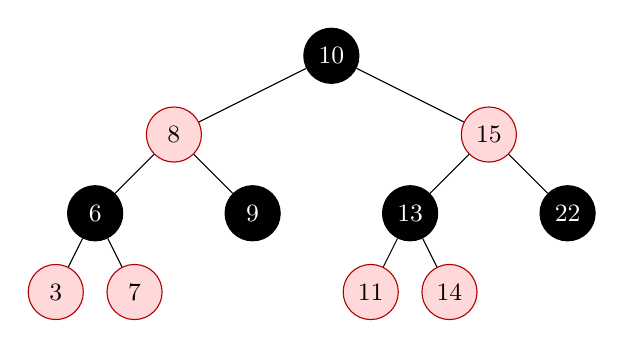
\begin{tikzpicture}[level distance=10mm,
  b/.style={circle,draw,fill=black,text=white,inner sep=1pt,minimum size=7mm,font=\small},
  r/.style={circle,draw=red!70!black,fill=red!15,inner sep=1pt,minimum size=7mm,font=\small},
  level 1/.style={sibling distance=40mm}, level 2/.style={sibling distance=20mm},
  level 3/.style={sibling distance=10mm}]
\node[b] {10}
  child {node[r] {8}
    child {node[b] {6} child {node[r] {3}} child {node[r] {7}}}
    child {node[b] {9}}}
  child {node[r] {15}
    child {node[b] {13} child {node[r] {11}} child {node[r] {14}}}
    child {node[b] {22}}};
\end{tikzpicture}
\end{center}
檢查：每條根到 \textsc{nil} 的路徑都有 $2$ 個黑節點（不算 \textsc{nil}，例如 $10, 8, 6, 3$ 是 $10, 6$；
$10, 8, 9$ 是 $10, 9$），沒有紅節點有紅子。

逐項檢查：
\begin{itemize}
\item (A) 紅節點是 $8, 3, 7, 15, 11, 14$，共 $6$ 個。 對。
\item (B) $8$ 是紅的。 錯。
\item (C) $14$ 是紅的。 對。
\item (D) $7$ 的父節點是 $6$（插入 $6$ 時的旋轉把 $6$ 放到 $3$、$7$ 上面）。 錯。
\item (E) $10$ 的子節點 $8$、$15$ 都是紅的（$15$ 在插入 $14$ 時改紅）。 對。
\end{itemize}
\end{pastsoln}
